\documentclass[12pt, titlepage]{article}

\usepackage[sumlimits,nointlimits,namelimits]{amsmath}
\usepackage{amsfonts}
\usepackage{amssymb}
\usepackage{mathtools}
\usepackage[shortlabels]{enumitem}
\usepackage{graphicx}

\usepackage[utf8]{inputenc}
\usepackage[T1]{fontenc}
\usepackage{lmodern}
\usepackage[margin=1in]{geometry}
\usepackage{fancyhdr}
\usepackage[dvipsnames]{xcolor}
\usepackage{tikz}

\usepackage{tikz}
\usetikzlibrary{shapes.geometric, arrows, positioning, fit}

\setlist[itemize]{topsep=0pt}
\setlist[enumerate]{topsep=0pt, label=(\alph*)}

\setlength\parindent{0pt}
\setlength\parskip{6pt}

\renewcommand{\headrulewidth}{0pt}
\fancyhead[L]{\bf CS 452/652}
\fancyhead[C]{\bf Train Control 1}
\fancyhead[R]{\bf Heun \& Yao}

\usepackage{hyperref}

\hypersetup{
    pdftitle={Train Control 1}
    colorlinks=false,
    pdfborder={0 0 1.5},
    linkbordercolor=red,
    urlbordercolor={0 1 1}
}

\usepackage{environ}
\makeatletter
\newsavebox{\measure@tikzpicture}
\NewEnviron{scaletikzpicturetowidth}[1]{%
  \def\tikz@width{#1}%
  \def\tikzscale{1}\begin{lrbox}{\measure@tikzpicture}%
  \BODY
  \end{lrbox}%
  \pgfmathparse{#1/\wd\measure@tikzpicture}%
  \edef\tikzscale{\pgfmathresult}%
  \BODY
}
\makeatother

\begin{document}
    \begin{titlepage}
        \begin{center}
            \vspace*{5em}
            \textbf{\LARGE Train Control (Part 1)}
            \vspace*{3em}

            \begin{tabular}{c@{\hskip 8em}c}
                \textbf{\large Niclas Heun} & \textbf{\large Trevor J. Yao} \\
                {\small nheun@uwaterloo.ca} & {\small t27yao@uwaterloo.ca} \\
                {\footnotesize 21111245} & {\footnotesize 20830290} \\
            \end{tabular}

            \vfill

            Professor Ken Salem \\
            CS 452/652: Real-Time Programming (Fall 2023) \\
            University of Waterloo \\
            9 November 2023

            \vspace*{5em}

        \end{center}
    \end{titlepage}


    \pagestyle{fancy}

    \tableofcontents
    \listoffigures
    \pagebreak

    \section{Overview}
    \label{sec:overview}

    This assignment begins the implementation of the complex real-time problem of train control. In order to accurately route and stop trains on arbitrary positions on the track, our train control program runs atop the kernel which we have built over the last month. The user interface is built upon the K4 UI, adding a few additional interactive commands to route trains between arbitrary positions on the track. All the commands to interact with the track are as follows:

    \begin{itemize}
        \item \verb`tr <train number> <train speed>`: Set the speed of the specified train. The train number must be a valid supported train (i.e. listed in the interface), and the speed must be an integer in the range $[0,14] \cup [16,30]$, where the latter is used to toggle the light status.
        \item \verb`rv <train number>`: Change the direction of the specified train to reverse. When run, the train will stop, before reversing at the same speed as before. Preserves the status of headlights.
        \item \verb`sw <switch number> <switch direction>`: Throw the given switch in the given direction (\verb`s`/\verb`S` or \verb`c`/\verb`C`). The switch number must exist on the track
        \item \verb`tc <start> <end> <offset> <train number> <speed>`: Route the specified train from the start to end track nodes, stopping offset mm after (if positive) or before (if negative) at the specified speed. The track nodes must match their names in the track data (i.e. case sensitive). The speed is specified as one of \verb`lo`/\verb`med`/\verb`hi`. Note that the start node must be in the forward direction of the train.
        \item \verb`st <train number>`: Stops the train mid-route. Useful for force quitting.
        \item \verb`go`: Send the `Go' signal to the track.
        \item \verb`hlt`: Send the `Stop' signal to the track.
        \item \verb`q`: Halt the program and return to boot loader. This will send any remaining commands to the track before stopping control.
    \end{itemize}

    Note that our implementation differs from the assignment specification in the omitance of the requirement to route the trains to a loop and wait for constant speed and throw all the switches in the requested route. It rather routes from a starting switch and end switch and throws switches only when necessary.

    \subsection{Submission SHA}

    The repository for the kernel is \href{https://git.uwaterloo.ca/t27yao/cs452-kernel}{ist-git@git.uwaterloo.ca:t27yao/cs452-kernel.git}. The submission SHA is fcd593a3fde7dffb3e00694ad7551ac8998de734.

    \subsection{Program Structure}

    The program (including the kernel) is structured into three sections. The \verb`kernel/` directory contains all the kernel code, including task descriptors, syscall/interrupt handlers, context switching functions, program execution timers, and allocators for task descriptors and stacks.

    The root directory \verb`include/` and \verb`src/` directories contain system library code, which is used by user-level programs to interact with the kernel, and also any shared data structures between the kernel and user programs. These include interfaces for using any kernel-provided functionalities (i.e. syscalls, interrupt events, message passing). The interfaces for interacting with the Raspberry Pis, as well as assorted utility functions (string/memory interactions) are also found in the system library, and are used by both the kernel and user-level programs. The system library directory also holds the implementation of user-level servers, including the Name Server, Clock Server, and two I/O Servers, as well as their respective APIs. Finally, the system library also contains the deque (double-ended queue) and binary heap data structures.

    All the user-level code needed to implement train control is contained in the \verb`track-control/` directory.\footnote{It was only realised when writing this document that this directory was indeed misnamed.} The contents of this directory are all discussed in detail throughout this document.

    \section{Execution}

    The Train Control program can be built from the root directory by running \verb`make` or \verb`make all`. It may be necessary to set the \verb`XDIR` variable to point to the directory containing the cross-compiler. For example, in the \verb`linux.student.cs` environment, \verb`XDIR` should be set to \verb`/u/cs452/public/xdev` (i.e. the parent of the \verb`bin` directory). Therefore, the program can be compiled in the \verb`linux.student.cs` environment by changing directory to the program root and executing:
    \begin{verbatim}
make XDIR=/u/cs452/public/xdev
    \end{verbatim}

    % A description of your work for this assignment. It should explain how you route the train, and how you get the train to stop at a target location. It should describe how you are modeling the train, including a description of any calibration data you have collected for modeling, and a description of how it was collected. Finally, it should describe how your train control system is implemented. In particular, it should describe the purpose and design of any tasks that are running, and their priorities. If you have made any modifications to your kernel to support TC1, explain those as well.

    \section{Calibration}
    \label{sec:calibration}
    For this assignment, we collected data on 4 metrics: constant speed, acceleration, deceleration, and stopping distance. In particular, we measured constant speed velocity for the trains at three speeds, giving the train control speeds \verb`hi`, \verb`med`, and \verb`lo`, corresponding to speeds 11, 9, and 7 respectively. Acceleration and deceleration data was gathered between the lowest speed and the two other speeds, as well as from a stopped train accelerating to the lowest speed. The stopping distance was also measured for all speeds. The raw data measured during calibration tests is stored in \verb`docs/tc1/data.txt`, along with the result of calculations done to produce the desired result (velocity, acceleration, stopping distance). The sanitised data is accessed throughout the program via the \verb`speed_data` structure (defined in \verb`track-control/include/speed-data.h`), and is initialised in the \verb`speed_data_init` method.

    \subsection{Collection Methods}

    All data was collected on Track B to ensure consistency, and we later found that no adjustments were needed to our model when executing on Track A. All calculations were done programmatically in C via a calibration program on our kernel, to account for any delays which may occur during actual train control while running on our kernel. Since our calculations were done in the calibration program itself, we may have had some rounding errors, since the Raspberry Pis do not support floating point arithmetic. However, we accounted for these by scaling distance so that we always used micrometres ($\mu m$) as our distance unit, rather than the less accurate millimetre unit. Finally, we removed as much sensor delay as possible by only polling single sensor modules when sensor activations were needed. The calibration programs can be found in the \verb`track-control/tests/calibration/calibration-test.c` file.
    
    We originally performed constant speed measurements on all the trains on the track, and used this to select a pool of trains with consistent speed profiles, in regard to itself and the other selected trains. This resulted in us using Trains 24, 58, and 77. We then also had to retake these constant speed measurements as we were seeing inconsistent results when moving onto the acceleration and deceleration data calibration, and removed the as much timing overhead as possible.
    
    The measurements were done in a self-hoisting manner, by first measuring velocity at constant-speeds, before using this data to calculate acceleration/deceleration and stopping distance, and then using the stopping-distance data to make measuring acceleration from zero easier.

    \subsubsection{Constant Speed}
    \label{sec:constant-speed}
    
    We measured all the trains between sensors E12 and C16 at a constant speed, giving at least one loop between any speed changes. We used this larger loop to try and ensure speed consistency, and used this stretch of track in order to understand how the speed of the trains differed inside the banked curve and on the straight. For each speed, after discarding the first loop, we looped the track 10 times, measuring the time between the sensor activations of the start and end sensors. We then calculated the velocity for each loop via the formula
    \[
        v = \frac{d \times 10^9}{t},
    \]
    scaling the given millimetre distance from the track data to obtain our velocity in $\mu m / s$.
    
    \subsubsection{Acceleration \& Deceleration}
    \label{sec:accel-decel}
    
    For acceleration and deceleration, we used a slightly longer stretch of track in order to properly capture the change in speed, and give ourselves room to make sure that the time the train reached the second velocity was indeed within our measuring distance. As we did in the constant-speed velocity measurements (Section \ref{sec:constant-speed}), we used the large loop in order to get a good straight-line measuring distance. Each train then after tripping the first sensor, accelerates to higher speed, and completes a loop, before tripping the first sensor again and decelerating back to the original speed. This is done for all trains with speed pairs $(7, 9)$ and $(7, 11)$, between sensors E13 to D13 and E13 to C6 respectively, 10 times each. 
    
    Using the measured time between their respective sensors, we calculated $t_x$, the time at which the train is estimated to have reached the secondary velocity by rearranging the formula $\overline{v} t_x + v_2(t - t_x) = d$ to calculate $t_x$ as follows:
    \[
        t_x = 2 \frac{d - v_2 t}{\overline{v} - v_2} = 2 \frac{d-v_2t}{v_1 - v_2} = \frac{2(d \times 10^9 -v_2t)}{v_1 - v_2}
    \]
    after scaling the distance, and then calculating the actual velocity as follows (again, after scaling):
    \[
        a = \frac{10^6(v_2 - v_1)}{t_x}.
    \]
    This was done for each acceleration time and averaged, and separately for the deceleration times.

    \subsubsection{Stopping Distance}
    
    For stopping, it was decided to use a sensor which is on the start of a gentle bank to get an average between the sensors on straights and those on more curved banks. For this, we chose C6. We measured stopping distance by using a binary-search like program to find a suitable delay after triggering the start sensor E12 that resulted in us stopping directly at the sensor. We used to start of the train pickup as our desired stopping point, and faced all trains so that the pick up was at the front. After having found the desired delay $t_d$, we calculated the stopping distance as
    \[
        d_s = \frac{d \times 10^6 - vt_d}{10^3},
    \]
    after scaling, resulting in $\mu m$ as desired.

    \subsubsection{Acceleration from zero}
    
    Acceleration from zero was a special case of acceleration (Section \ref{sec:accel-decel}), and used the previously calculated stopping distance data to stop the train  directly at the first sensor, and measuring the time after sending the speed-up command and triggering the end sensor. This was done between sensors D11 and C6 to avoid issues with trains getting stuck on the track at lower speeds.

    \section{Modelling}
    \label{sec:modelling}
    
    In order to avoid rounding errors during the calibration process (Section \ref{sec:calibration}), all distances were stored in terms of micrometres ($\mu m$). Given this, our modelling functions also keep precision by using micrometres for any distance units, and using clock-server ticks as the time unit, since that is how our tasks understand ``time''. In other words, we use $\mu m$ for distance, $\mu m / s$ for velocity, and $\mu m / s^2$ for acceleration. The \verb`speed_data` singleton class offers a range of methods which calculate distance and time of trains based other kinematics variables for all stages of a train while on route (i.e. acceleration, constant speed, and stopping). 
    
    \subsection{Constant Speed}
    \label{sec:modelling-constant}
    
    Given the speed of the train, we often want to calculate how far the train will have travelled in a given time (assuming the train's speed has stayed constant). This is calculated via
    \[
        d = \frac{vt_{ticks}}{10^2},
    \]
    where $v$ is the calibrated velocity of a train moving at the given speed. Note that in order to scale the clock server ticks, we need to divide by a factor of $100$, since a clock tick is a 10ms unit.
    
    Its complementary function calculates the time needed to travel a specified distance at the current speed. This is used for calculating the expected time of arrival at the next sensor
    \[
        t_{ticks} = \frac{d \times 10^2}{v}.
    \]

    \subsection{Acceleration}
    
    As for constant speed, we require the distance and time a train will take to accelerate between speeds. However, if the train is currently accelerating between speeds, the constant model above fails. In this case, we are able to model this scenario via a linear acceleration mode. We are able to find the distance via the following formula:
    \[
        d = \frac{1}{2} \frac{v_2^2 - v_1^2}{a}.
    \]
    Moreover, we are able to approximate the time it takes for the train to change speeds via
    \[
        t_{ticks} = \frac{(v_2 - v_1) \times 10^2}{a}
    \]
    
    \subsection{Stopping}
    
    In order to accurately stop, since we know the distance required for a train to stop at a certain speed (from our calibration work in Section \ref{sec:calibration}), we must calculate how long we must delay after activating one of the sensors prior to the stopping point before sending the brake command. Using the constant speed models (Section \ref{sec:modelling-constant}), we are able to calculate this delay time using the known distance from the ``activation sensor'' and the target via our constant time model:
    \[
        t_{delay} = \frac{(d_{total} - d_{stop}) \times 10^2}{v},
    \]
    where $v$ is the velocity the train was travelling at.

    \section{Routing}
    \label{sec:routing}
    
    Trains find a path from the specified source and destination nodes via the \verb`plan_route` method contained in \verb`track-control/include/routing.h`. This header also provides the interface for the \verb`routing_action` and \verb`routing_action_queue` classes, which enable the routing algorithm to communicate actions (i.e. switches to throw, speed changes, sensor to wait on, etc) to the Train Administrator (Section \ref{sec:train}).
    
    A \verb`routing_action` is an action that the train administrator must perform in order to move the train on the track. It consists of a sensor (or possibly none), an action (throwing a switch, changing speed, reaching a sensor, or reaching constant speed), and possibly a time delay that must pass after the sensor activation (if any) before the action is performed. For example, a switch throw is usually tied to a previous sensor activation, and does not need to delay. However, for close sensors on initial acceleration, the switches which need to be thrown are not tied to any sensor activation. Initial acceleration commands are not tied to any sensor activations, but tied only to time offsets (see Section \ref{sec:train}), but the stopping command needs to be tied to both a sensor activation and a time offset to stop directly where desired.
    
    The \verb`routing_action_queue` allows the routing algorithm to communicate a plan for routing via \verb`routing_action` structures. The queue is actually double-ended, and built atop the regular deque, which is more than fast enough for our purposes, and the wrappers ensure data consistency.
    
    To simply our discussion, we will first discuss the \verb`plan_direct_route` helper function, which searches for a route in the forward direction, and is the main driver of the algorithm. This method makes use of two \verb`routing_action_queue`'s, one for speed actions and one for path actions (sensors in the path, switches, etc). In general, routing and train algorithms split actions into speed actions and path actions. This is to save on modelling calculations, since there is a relative ordering between actions in their respective domains. The actual \verb`direct_route` method checks first for a direct forward route and if that fails, attempts a backwards route, adding the required reverse commands at the start and end, adjusting the offset to maintain the same front axle stopping target, and ensuring that the forward sensor is not actually added to the path, since the train will be reversing.
    
    The routing algorithm is a modified Dijkstra's Algorithm\footnote{\url{https://en.wikipedia.org/wiki/Dijkstra's_algorithm}} on the \verb`track_node` digraph. To enable this algorithm, we use a minimum binary heap priority queue to store graph weights, implemented in \verb`include/priority-queue.h`. This priority queue provides in place linear construction of the heap from an array, adding with priority, logarithmic time removal of the lowest priority element, and logarithmic decrease of priority, the minimum methods needed to implement Dijkstra's algorithm.
    
    Our algorithm differs from Dijkstra's Algorithm by also terminating if we reach the reverse node. Before backtracking to construct the path, it also checks based on our train model (Section \ref{sec:modelling}) if we have enough space on the path (i.e. distance) to accelerate to the requested speed, roll at constant speed to ensure consistent stopping distance, and then distance to stop. If not, the algorithm terminates early before constructing the path. Note that the ``rolling distance'' was chosen that a route can always be found on any two nodes on the track if the backwards and forwards distance is attempted, while allowing suitable distance to stay at constant speed.
    
    The algorithm also differs from the standard Dijkstra's Algorithm in the backtracking path finding, since it needs to create routing actions, rather than path nodes. It ignores all nodes except branch and sensor nodes. Branch nodes are pushed onto a queue in order to find a suitable sensor (if any) that the switch should be thrown at. Then, for each sensor node, we check if it a suitable distance from a queued branch node (via the calculated distances used in the pathfinding portion of Dijkstra's Algorithm), and if so, adds a routing action which waits on the sensor and throws the switch. Note that one node may have multiple switches to throw. The suitable distance is found by calculating the distance the train will travel at the desired speed in 3 seconds, via our model (Section \ref{sec:modelling-constant}). Note that this minimum time can be much decreased without impacting routing, but we found that stopping distance could be smaller time offsets.
    
    Stopping distance nodes are found similarly, but only once, since we are backtracking, and compared to the calibrated stopping distance. Finally, for each node the algorithm also adds a sensor wait which also contains the distance to the next node (which is easily known since we are backtracking). This is what allows the Track Control Coordinator (Section \ref{sec:tcc}) to make position predictions. This means that the Train Administrator (Section \ref{sec:train}) often will wait on sensors without any actions. However, since we are backtracking, this wait is always the first routing action for a given sensor, allowing the Train to efficiently perform multiple actions per switch activation, while allowing us to backtrack efficiently in a single linear pass.
    
    Finally, after we have found a path, we add any leftover branch switches which did not have enough distance for an activation sensor to the path queue, to be thrown immediately without any delay. We also use our acceleration model to calculate the time needed to accelerate to first the \verb`LO` speed, and then the specified speed, if higher than \verb`LO`. This two stage acceleration is necessary since we decided only to model acceleration from zero to speed \verb`LO` to save time. 
    
    Our routing algorithm is incredibly efficient even with a double path-find on a large digraph, since we terminate early. In our tests, the average execution time was 1.5ms, with a worst case of 3ms. This makes it more than suitable for performing the constant path recalculations needed in TC2. Moreover, for implementing collision avoidance, the routing algorithm could be easily adapted to query an external track server which manages the track distance weights, in order to reroute around blocked paths.

    \section{Train Control Design}
    The Train Control program is divided into five main components:
    \begin{itemize}
        \item Program Tasks (\verb`track-control/include/program-tasks.h`);
        \item Track Control Coordinator (\verb`track-control/include/track-control-coordinator.h`);
        \item Sensor Worker (\verb`track-control/include/sensor-worker.h`);
        \item Train Administrator and Notifiers (\verb`track-control/include/train.h`);
        \item Märklin Server (\verb`include/marklin-server.h`);
        \item Console Server (\verb`include/console-server.h`).
    \end{itemize}
    
    \begin{figure}[h]
    \resizebox{0.95\textwidth}{!}{
    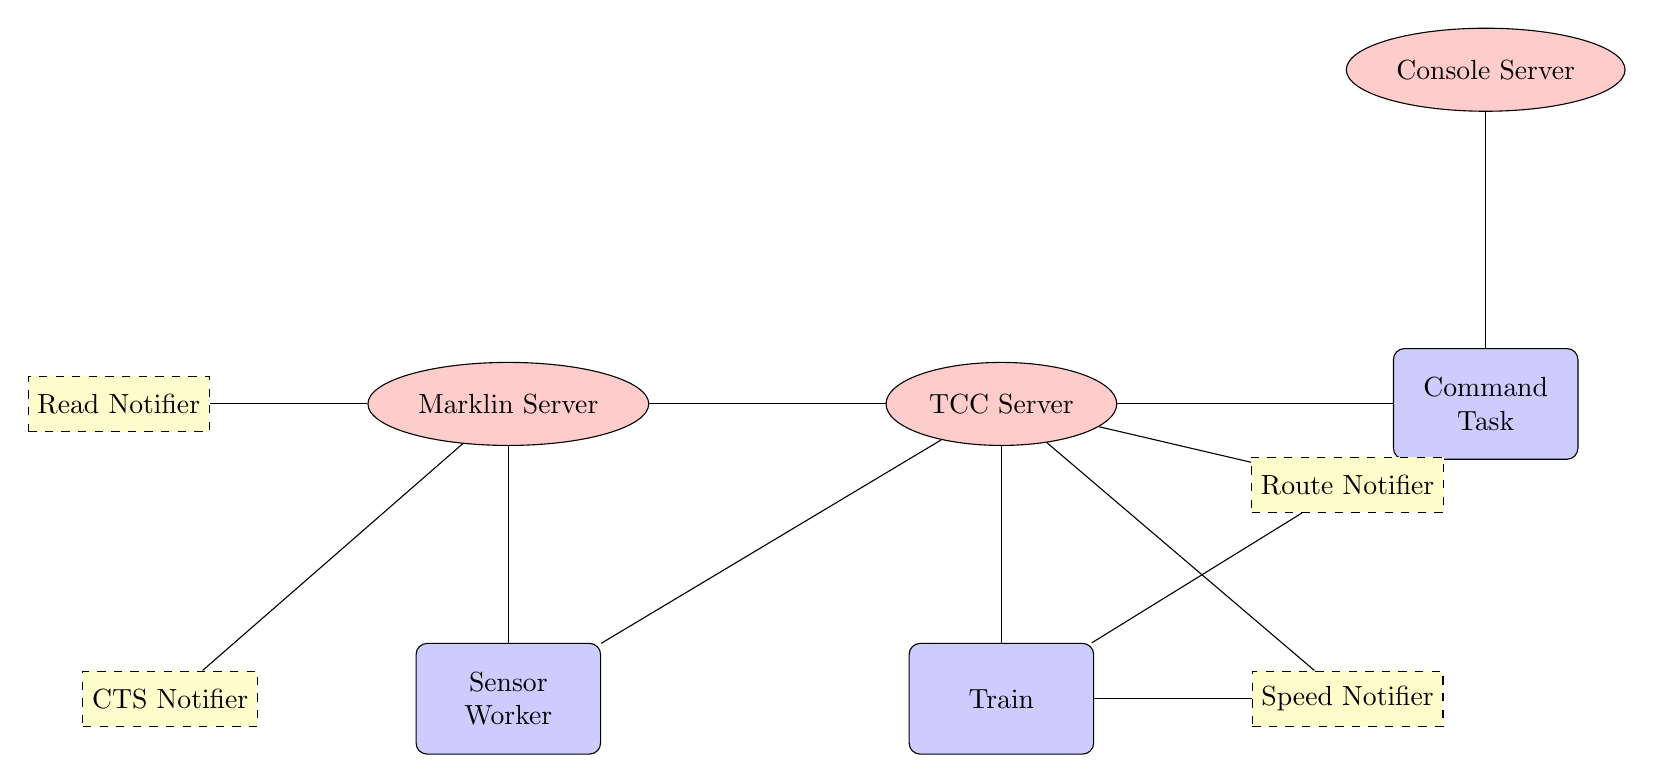
\begin{tikzpicture}[node distance=2.5cm and 3.5cm, auto]

        % Define styles
        \tikzstyle{block} = [rectangle, draw, fill=blue!20, text width=6em, text centered, rounded corners, minimum height=4em]
        \tikzstyle{cloud} = [draw, ellipse,fill=red!20, node distance=3cm, minimum height=3em]
        \tikzstyle{line} = [draw]
        \tikzstyle{notif} = [draw, rectangle, dashed, fill=yellow!20, node distance=2cm, minimum height=2em, text centered]
    
        % Place nodes
        \node [cloud] (marklin) {Marklin Server};
        \node [block, below=of marklin] (sensorworker) {Sensor Worker};
        \node [cloud, right=of marklin] (tcc) {TCC Server};
        \node [block, right=of tcc] (program) {Command Task};
        \node [cloud, above=of program] (console) {Console Server};
        \node [block, below=of tcc] (train) {Train};
    
        % Notifiers
        \node [notif, left=of marklin] (Read) {Read Notifier};
        \node [notif, left=of sensorworker] (ctsnotif) {CTS Notifier};
        \node [notif, right=of train] (speednotif) {Speed Notifier};
        \node [notif, above=of speednotif] (routenotif) {Route Notifier};
    
        % Draw edges
        \path [line] (console) -- (program);
        \path [line] (marklin) -- (sensorworker);
        \path [line] (marklin) -- (tcc);
        \path [line] (sensorworker) -- (tcc);
        \path [line] (tcc) -- (train);
        \path [line] (program) -- (tcc);
        
        % Notifier connections
        \path [line] (Read) -- (marklin);
        \path [line] (ctsnotif) -- (marklin);
        \path [line] (speednotif) -- (train);
        \path [line] (routenotif) -- (train);
        \path [line] (speednotif) -- (tcc);
        \path [line] (routenotif) -- (tcc);
    
    \end{tikzpicture}
    }
    \caption{Train Control Tasks}
    \end{figure}
    
    The \emph{Program Tasks} refer to a collection of user-level tasks which handle Console Interaction. These tasks handle UI elements such as the displayed clock and idle time in the console, as well parsing user inputs. These are discussed more in detail in the Kernel Documentation as part of the K4 Assignment. Note that the parsing algorithm was adapted to parse the names of any track nodes specified by the user and determine where on the track node it lies without a linear search, making an efficient start-up.
    
    The \emph{Track Control Coordinator} (TCC) coordinates all actions involving the track, and has knowledge about all actions happening on the track. This includes sensor activations, train positions, train speeds, etc. The TCC acts as an intermediary between the Märklin Server and any tasks wanting to send/receive information to/from the track. The \emph{Sensor Worker} is the only process reading data from the Märklin, on behalf of the TCC.
    
    Every train is represented by a \emph{Train Administrator} during the duration of its routing on the track. All actions required to route the train between points (such as speed changes or thrown switches) are sent directly the TCC when appropriate, which is determined by the routing algorithm, and carried out by the notifiers on behalf of the administrator. As the intermediary, the TCC applies them towards the track, and also helps to determine 

    The \emph{Märklin} and \emph{Console} Servers are unchanged from the K4 Assignment, and are described in more detail in that documentation. They handle sending and receiving from the Märklin and Console respectively. 
    
    \subsection{Track Control Coordinator}
    \label{sec:tcc}
    
    The \emph{Track Control Coordinator} is inspired by an Air Traffic Control Tower and designed with TC2 and multiple trains in mind. It has full authority over the tracks, and has knowledge on all switch/sensor states, along with any trains in progress on the track. It offers the following interface to trains (Section \ref{sec:train}):
    \begin{itemize}
        \item Registering a train;
        \item Deregistering a train;
        \item Set/Get train speed;
        \item Set a switch;
        \item Wait for a specific switch to be activated. 
    \end{itemize}
    
    For this part, the TCC only stores changes in state and sends any requested actions to the Märklin Server. In the next part of this assignment, the TCC will become responsible for modifying, delaying, or even possibly denying requests to trains in order to maintain separation between trains with conflicting goals. It also allows processes to block on various sensor activations, and these waiting processes are managed using the Sensor Queue (Section \ref{sec:sensor-queue}) data structure. Lastly, the TCC is responsible for calculating the expected time the next sensor will trigger for a given train, and comparing this expected value to the true value which it recorded. We decided to incorporate this into the TCC, since it is the only task which has knowledge of the state and expected state of all trains, and is able to react to unexpected states.

    \subsubsection{Sensor Queue}
    \label{sec:sensor-queue}
    
    The \emph{Sensor Queue} is maintained by the TCC to keep track of all processes waiting for a specified sensor activation (or any).
    It is implemented as an intrusively linked list indexed by a 2D array of size \verb`N_SENSOR_MODULES` $\times$ \verb`N_SENSOR_PER_MODULE`, which maintain the head pointer to the queues for each sensor.
    Like the many queues in the kernel, it is implemented via a freelist of free nodes with stack-allocated storage.

    Whenever a new process waits for a sensor activation, an entry is taken from the free list and enqueued for the specific sensor on the 2D array. Then, on any subsequent sensor activation, all waiting processes on the given sensor are dequeued. 

    \subsection{Sensor Worker}
    \label{sec:sensor-worker}
    
    The \emph{Sensor Worker} is owned by the TCC server, and is responsible for reading sensor data coming from the track, which it also queries. This is done to prevent the TCC from blocking, and allow it to continue to receive requests from other tasks. Like in K4, the task waits for the output queue of the Märklin Server to become empty, and continually queries the Märklin controller whenever no commands are being sent. From this, it reads and parses the data, sending any activations to the TCC, which can deque any waiting processes.

    \subsection{Positioning}
    \label{sec:positioning}
    
    One of the must critical responsibilities of the TCC is comparing the predicted sensor activation time with the actual sensor activation time (and thus predicted/actual positions).
    These methods are implemented in the \verb`track-control/include/position.h`.
    In our implementation, the Train (Section \ref{sec:train}) waits for every sensor activation on the route, so that the TCC knows where the train wants to go. In this information, it also provides data on the distance to it's next sensor.
    On the sensor activation, we store the timestamp of the activation and compare it with the last sensor activation for this train. 
    By considering the distance and expected velocitay, we can compute the difference in expected and actual train position.
    
    However, calculating the expected position when taking into account the speed changes (i.e. acceleration from zero, stopping) between sensor activations is a challenging problem. Even though we have an acceleration model, we were only able to get rough estimates, and the situation where the trains accelerated over multiple sensors was not accurate. For simplicity in this assignment, we calculate the position assuming constant velocity. Since we start the train from zero, the first few estimates are inaccurate since we are accelerating rather than at our constant peak speed. However, we have found that the constant speed estimates reflect reality.

    \subsection{Train Administrator}
    \label{sec:train}
    
    The \emph{Train Administrator} (\verb`track-control/include/train.h`) is a short lived task (i.e. exits after it's prescribed work has completed) which is responsible for obtaining a route (via the Routing Algorithm -- Section \ref{sec:routing}) and executing the planned route, both by throwing the prescribed switches as the train travels along the route, and changing the speed as modelled and calculated by the routing algorithm. As previously mentioned, the plan is returned by the routing algorithm in two queues of \verb`routing_action` structs, corresponding to the path and the speed changes.
    
    After obtaining the plan, the administrator throws any initial switches at the start (who wait on no sensors) to ensure that we are ready to start. It then follows the instructions of each \verb`routing_action`, waiting for sensor activations (if prescribed) and delays (if needed) before executing the actual action. The administrator only waits for one action trigger per queue, but for both queues. However, note that since we are required to block, and there is no strict ordering between speed events and path events, we make use of notifiers to wait on events as needed for each queue. This allows us to wait on events from both queues without worrying about strict ordering.

    \subsubsection{Train Notifier}
    \label{sec:train-notif}
    
    Both the Route Path and Speed queues have their own respective notifiers. These notifiers are the exact same, but differ in priority level, as well as behaviour after wait. The Speed Notifier executes the action on behalf of the train administrator, since there is only ever one event per wait, and the action is often very time sensitive. However, this does not hold true for the Route Notifier, since the Route queue often will have multiple actions waiting to be triggered on one sensor. Rather than passing multiple sensors, the administrator is able to wait on the first sensor trigger, and after the notifier finishes waiting on it's behalf, the administrator task executes all the actions on the queue which wait on the same sensor.
    
    When the Notifier (on behalf of the Administrator) waits for an event, it passes metadata to the Track Control Coordinator, allowing it to make position predictions (Section \ref{sec:positioning}). This metadata is also calculated at the routing level, allowing total separation between planning and actual execution.
    
    \subsection{Task Priorities}
    
    As documented in the Kernel documentation, we have the following non-idle priorities, listed from highest to lowest:
    \begin{itemize}
        \item Notifier;
        \item Server (HI);
        \item Server (LO);
        \item Very-High;
        \item High;
        \item Medium;
        \item Low.
    \end{itemize}
    Note that for more information on tasks mentioned in the priority listing below not referred to in this document, please consult to Kernel Documentation.
    
    The Clock Server Notifier, Märklin Notifiers (CTS/Read) and Console Read Notifier all run at the notifier priority. The Clock Server, Märklin I/O, and Track Control Coordinator (Section \ref{sec:tcc}) all run at the higher server priority, since they are more time sensitive to the Nameserver and Console I/O server, which run at the lower server priority.
    
    At the non-server level, the Train Speed Notifier (Section \ref{sec:train-notif}) runs at the highest Very-High level, since stopping accurately is very time sensitive. The Task responsible for the displayed system clock, along with the task used to reverse trains (after manual input), and the Sensor Worker (\ref{sec:sensor-worker}) all run at the High level, as other time sensitive tasks. However, we do not want to clog the train-control task. Finally, less time sensitive tasks such as the Train Route Notifier and any Train Administrators run at Medium Priority (since track switching is less time sensitive in our current application), as well as the Command Task, which parses slow user input. Finally, the task which update the Idle UI runs at the lowest priority, for obvious reasons.

    \section{Kernel Modifications}

    Two new system calls were added to enable two features of our Track Control UI. First, we added the \verb`GetIdleStatus` syscall for obtaining the current idle time and current total user execution time, to enable a user task to update the displayed idle ticks. Finally, we added the \verb`KillChild` syscall to allow Train Administrators (Section \ref{sec:train}) to be killed from the command line.
\end{document}
